\documentclass{scrartcl}
\usepackage[utf8]{inputenc}
\usepackage{hyperref}
\usepackage{url}
\usepackage{natbib}
\usepackage{graphicx}
\usepackage{cleveref} % this must be the last package to be loaded

\newcommand{\emailaddr}[1]{\href{mailto:#1}{\texttt{#1}}}

\title{\LARGE
    Distributed Lupus in Fabula
}
\subtitle{Final Report for the Distributed Systems Course 2025/2026}

% Consider watching:
% https://www.youtube.com/watch?v=ihxSUsJB_14
% https://www.youtube.com/watch?v=XTFWaV55uDo

\author{
    Jacopo Bonifazi \\ \emailaddr{author1@email.it}
    \and
    Alexandru Nicolescu \\ \emailaddr{author2@gmail.com}
    \and
    Leonardo Vorabbi \\ \emailaddr{leonardo.vorabbi@studio.unibo.it}
}

\date{\today}

\begin{document}

\maketitle

\begin{abstract}
  Distributed Lupus in Fabula is a real-time multiplayer web application that brings the classic social deduction game Lupus in Fabula online, allowing groups of players to create or join a game lobby from any browser and play a full match together over the internet.
  The system is composed of a Vue 3 single-page frontend and a FastAPI/Socket.IO backend, communicating via REST for stateless operations and via WebSocket for real-time, low-latency interactions such as votes, phase transitions, and private role actions. Game and lobby state is kept in Redis rather than a traditional database, acting both as a shared source of truth across backend replicas and as a Pub/Sub broker that lets events generated on one instance reach clients connected to any other instance.
  This design allows the backend to run as multiple concurrent, interchangeable replicas behind a reverse proxy, supporting many simultaneous matches while keeping every player's view of the game synchronized in real time.
\end{abstract}

\section*{Disclaimer}

During the preparation of this work, the authors used LLMs to to refine syntax and correct linguistic errors.

After using this tool, 
the authors reviewed and edited the content as needed 
and take full responsibility for the content of the final report/artifact

\section{Concept}\label{Concept}

\subsection{Type of Product}

The project is a web application, specifically a real-time multiplayer game inspired by the traditional social deduction game \textit{Lupus in Fabula}. It is a full-stack distributed system composed of:

\begin{itemize}
    \item A \textbf{frontend}: a Vue 3 Single Page Application (SPA), accessible via browser.
    \item A \textbf{backend}: a set of stateless, horizontally replicated web services built with FastAPI and Socket.IO, responsible for game logic, session management, and real-time event propagation.
    \item A \textbf{shared data layer}: Redis, used both as a low-latency state store and as a Pub/Sub message broker connecting the backend replicas.
\end{itemize}

The whole system is designed to be deployed as a multi-container distributed application, rather than as a single monolithic server.

\subsection{Use Case Description}

\paragraph{What the software does.}
The application lets a group of players create or join a virtual ``lobby,'' wait until everyone is ready, and then play a phase-based game of hidden roles and social deduction. Once a match starts, the game state moves automatically through a fixed sequence of phases:

\[
\textbf{LOBBY} \rightarrow \textbf{DAY} \rightarrow \textbf{VOTING} \rightarrow \textbf{NIGHT} \rightarrow \cdots \rightarrow \textbf{ENDED}
\]
driven by server-side timers.

During DAY/VOTING, players discuss and vote to eliminate a suspect; during NIGHT, players with special roles perform hidden actions that are resolved by the server before the next day begins. The match ends automatically once a win condition is met.

\paragraph{Where the users are.}
Players are geographically dispersed (or at least not necessarily co-located): each player connects independently from their own browser, over the public Internet, to a shared game session identified by a room/lobby code.

\paragraph{When and how frequently they interact.}
Interaction is continuous and real-time for the whole duration of a match (several minutes to tens of minutes), not just at fixed request/response intervals. Players must react within phase time limits (e.g., voting windows, night-action windows), so the system needs low-latency, event-driven communication rather than simple periodic polling.

\paragraph{How they interact.}
All interaction happens through a web browser via the Vue SPA. The frontend communicates with the backend in two complementary ways:

\begin{itemize}
    \item \textbf{REST} calls for stateless operations such as creating a lobby, joining a lobby, or fetching the current game state.
    \item \textbf{WebSocket} for real-time, bidirectional events: votes, phase changes, chat, private role actions, disconnect/reconnect notifications, etc.
\end{itemize}

\paragraph{Does the system store user data? Which, and where?}
The system does not use a persistent relational database for user accounts since there is no long-term profile storage. Instead, it relies on Redis as a shared, TTL-based store for all session-scoped game data:

\begin{itemize}
    \item room/lobby state and configuration;
    \item the list of connected players and their ready status;
    \item assigned roles (Wolf, Seer, Villager);
    \item votes cast during the DAY/VOTING phase and private night actions;
    \item phase timers and current phase;
    \item host identity.
\end{itemize}

On the client side, the browser itself retains a minimal amount of session data in local storage, purely to support reconnection and continuity of a player's session across page reloads or brief disconnects.

\begin{figure}
    \centering
    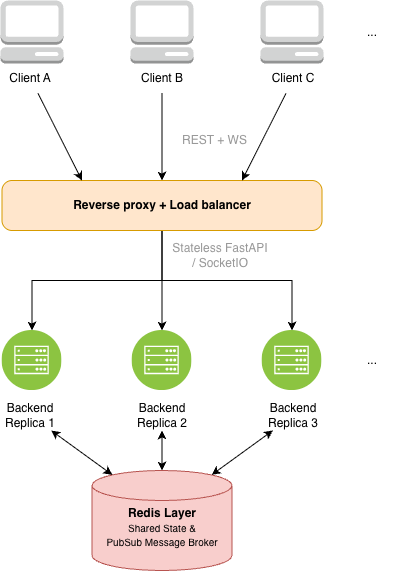
\includegraphics[width=0.40\textwidth]{figures/system_architecture_overview.png}
    \caption{High-level architecture: clients connect through a reverse proxy to stateless backend replicas, which share game state and propagate events through Redis.}
    \label{fig:architecture}
\end{figure}

\paragraph{Roles.}
The system distinguishes several actor roles at different levels:

\begin{itemize}
    \item \emph{Application-level roles}: \textbf{Villager}, \textbf{Wolf}, \textbf{Seer}, each with different permitted actions and visibility (e.g., Wolves share a private night chat, the Seer can inspect one player per night).
    \item \emph{Session-level roles}: the \textbf{Host}, who configures the match, can remove players from the lobby, and starts the game; versus \textbf{regular players}, who can only join, ready up, vote, and act according to their assigned role.
    \item \emph{System role}: the backend itself acts as an autonomous \textbf{orchestrator}. It owns the authoritative game state, advances phases via timers, resolves votes and night actions, and enforces which actions are legal at any given moment.
\end{itemize}

\subsection{Why Distribution Is Needed}

Distribution in this project is not motivated by geographic proximity to users, but primarily by scalability, real-time synchronization, and fault tolerance:

\begin{itemize}
    \item \textbf{Horizontal scalability / resource sharing.} The backend is designed to run as multiple stateless replicas behind a reverse proxy, so that many concurrent lobbies and matches can be served in parallel without a single process becoming a bottleneck. Because game state lives in Redis rather than in each process's memory, any replica can handle requests for any room, allowing the system to scale out simply by adding more backend instances.

    \item \textbf{Shared state across replicas.} Since each backend instance is stateless with respect to game data, Redis acts as the single source of truth for lobby/game state. This is what makes horizontal scaling actually work: a player's WebSocket connection can be handled by one replica while another replica processes a REST call for the same match, and both see a consistent view of the state.

    \item \textbf{Cross-replica real-time propagation.} Because clients belonging to the same room can be connected to different backend replicas, a simple in-process event emitter is not sufficient. The system uses Redis Pub/Sub to broadcast game events (vote updates, phase transitions, chat messages, etc.) across all replicas, ensuring that every client in a room receives updates regardless of which instance generated them or which instance is handling their socket.

    \item \textbf{Fault tolerance and continuity.} The backend includes explicit mechanisms for reconnecting to Redis, retrying failed operations, sweeping/recovering timers, and reconciling state after temporary inconsistencies (anti-entropy). This matters because a real-time game cannot simply crash or stall if a single backend replica fails, a Redis connection drops momentarily, or a player's browser disconnects and reconnects mid-match. The match state and timers must survive these events.

    \item \textbf{Reduced dependency on a single instance.} Because the game state is decoupled from any specific process, a backend replica can be restarted, replaced, or scaled down/up without necessarily terminating ongoing matches, and a reconnecting player can resume their session against a different replica than the one they were originally connected to.
\end{itemize}

In summary, this system is distributed primarily to support many concurrent matches, keep real-time state synchronized across independent backend replicas, and remain resilient to instance failures and client disconnections.

\section{Requirements Elicitation and Analysis}\label{requirements}

This section specifies \emph{what} the system must do, independently of the specific implementation strategies later adopted. Requirements are grouped into functional, non-functional, and implementation requirements, each with a unique identifier and an associated acceptance criterion to be used during validation.

\subsection{Functional Requirements}

\begin{description}
    \item[FR1 -- Lobby creation.] The system shall allow a user to create a new game lobby by providing a valid nickname.\\
    \textit{Acceptance criterion:} given a valid nickname, the system creates a room, assigns it a lobby code, and redirects the user to the lobby screen.

    \item[FR2 -- Joining an existing lobby.] The system shall allow a user to join an existing lobby using a room code and a nickname.\\
    \textit{Acceptance criterion:} with a valid room code, the player enters the lobby and appears in the participant list; with an invalid code, the system displays an error.

    \item[FR3 -- Browsing open lobbies.] The system shall display to the user the list of currently available lobbies.\\
    \textit{Acceptance criterion:} the home screen shows only lobbies that are still joinable, periodically refreshed from the backend.

    \item[FR4 -- Host management.] The system shall designate a host for each lobby and restrict room-control operations to that host.\\
    \textit{Acceptance criterion:} only the host can modify lobby settings, remove a player, and start the match.

    \item[FR5 -- Ready status.] The system shall allow players to declare themselves ready or not ready within the lobby.\\
    \textit{Acceptance criterion:} each player's ready status is updated accordingly, and the match can only start once the minimum required conditions are met.

    \item[FR6 -- Match start and role assignment.] The system shall start a match when requested by the host and assign a role to each participant.\\
    \textit{Acceptance criterion:} at match start, every player receives a role and the match enters the expected phase sequence.

    \item[FR7 -- Game phase management.] The system shall support the phases LOBBY, DAY, VOTING, NIGHT, and ENDED.\\
    \textit{Acceptance criterion:} the system displays the current phase and automatically transitions to the next phase according to the game rules.

    \item[FR8 -- Voting and special actions.] The system shall allow players to vote during the day and allow special roles to perform night actions.\\
    \textit{Acceptance criterion:} votes and actions are accepted only during the correct phase and produce an update visible to the other clients.

    \item[FR9 -- In-game chat.] The system shall allow participants in a room to exchange messages.\\
    \textit{Acceptance criterion:} a message sent by a user appears to the other players of the same match without a page refresh.

    \item[FR10 -- Reconnection and session recovery.] The system shall allow a disconnected player to reconnect to the same match.\\
    \textit{Acceptance criterion:} if the client rejoins with the same identity and the same room code, it recovers the correct current match state.

    \item[FR11 -- Match end and result.] The system shall determine the winner and display the final results screen.\\
    \textit{Acceptance criterion:} when a victory condition is met, the system transitions to ENDED and displays the winning faction, the roles, and the final status of all players.
\end{description}

\begin{figure}
    \centering
    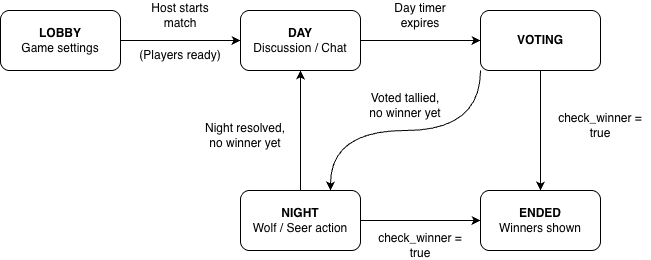
\includegraphics[width=0.9\textwidth]{figures/game_state_machine.png}
    \caption{State machine of the match phases. Transitions are driven automatically by server-side timers and by \texttt{check\_winner()}.}
    \label{fig:phase-state-machine}
\end{figure}

\subsection{Non-Functional Requirements}

\begin{description}
    \item[NFR1 -- State consistency.] The state of a match shall be consistent across all clients and across all backend replicas.\\
    \textit{Acceptance criterion:} two clients connected to the same room observe the same match state and the same host, even when served by different backend replicas.

    \item[NFR2 -- Availability.] The system shall remain usable even in the presence of a backend replica failure.\\
    \textit{Acceptance criterion:} if a backend replica goes down, clients can continue interacting with the match through the remaining active replicas.

    \item[NFR3 -- Fault recovery.] The system shall recover quickly from temporary disconnections of Redis or of a backend instance.\\
    \textit{Acceptance criterion:} after a temporary disconnection, the backend re-establishes the connection and clients receive the correct state again without the match being recreated.

    \item[NFR4 -- Responsiveness.] Player actions shall be visible to other participants in real time or near real time.\\
    \textit{Acceptance criterion:} votes, phase changes, chat messages, and reconnections are propagated without requiring a manual page refresh.

    \item[NFR5 -- Match data integrity.] The system shall not lose the current match state during normal operation.\\
    \textit{Acceptance criterion:} after restarting a single backend replica, the match state remains recoverable from the shared data store.

    \item[NFR6 -- Usability.] The interface shall allow a non-technical user to join and play a match without needing to understand the system's internal details.\\
    \textit{Acceptance criterion:} a user can complete lobby creation/joining, the lobby phase, and the match using only a browser and a room code.
\end{description}

\subsection{Implementation Requirements}

\begin{description}
    \item[IR1 -- Python backend.] The backend shall be implemented in Python using FastAPI and Socket.IO.\\
    \textit{Acceptance criterion:} the backend service exposes HTTP APIs and WebSocket/Socket.IO channels as specified by the design.

    \item[IR2 -- Web frontend.] The client shall be a Single Page Application built with Vue~3 and Vite.\\
    \textit{Acceptance criterion:} the application runs in the browser and communicates with the backend via REST and WebSocket.

    \item[IR3 -- Shared state on Redis.] The system shall use Redis as the shared store for lobby state, match state, votes, and timers.\\
    \textit{Acceptance criterion:} multiple backend replicas read and write the same state without relying on separate local data stores.

    \item[IR4 -- Containerized deployment.] The system shall be executable in containerized environments and support deployment via Docker Compose and Kubernetes.\\
    \textit{Acceptance criterion:} the full environment starts locally via Compose and can also be deployed on a Kubernetes cluster.

    \item[IR5 -- Observability.] The system shall expose metrics for monitoring purposes.\\
    \textit{Acceptance criterion:} the backend publishes metrics that can be queried by Prometheus and visualized in Grafana.
\end{description}

These constraints are consistent with the structure already adopted in the project repository: backend, frontend, Redis, reverse proxy, monitoring stack, and Kubernetes manifests.

\subsection{Features Less Relevant or Not Central}

\begin{itemize}
    \item \textbf{Geographical distribution.} This is not the main motivation for distribution in this project. The system is not designed for users spread across the globe requiring geo-aware routing or replication, but rather to support multiplayer gameplay and backend replication for scalability and fault tolerance.
    
    \item \textbf{Heterogeneity beyond the standard web stack.} This is not a strong priority. The system's components are built with different technologies (Vue, FastAPI, Redis), but all communicate through standard protocols (HTTP, WebSocket), and no complex integration with heterogeneous third-party systems is required.
    
    \item \textbf{Strong security model.} Security is not the main focus of the project. The system does not process critical personal data or financial transactions; security concerns are essentially limited to enforcing correct game actions and host privileges.
\end{itemize}

\section{Design}\label{design}

This chapter explains the strategies used to meet the requirements identified in the analysis. 
%
Ideally, the design should be the same, regardless of the technological choices made during the implementation phase.

\begin{quote}
You can re-arrange the sections as you prefer, but all the sections must be present in the end
\end{quote}

\noindent
\textbf{Important:} try to motivate your design choices in relation to the requirements and features identified 
in \cref{requirements} and \cref{ds-features}.

\subsection{Architecture}\label{architecture}

\begin{itemize}
  \item Which architectural style?
  %
  \begin{itemize}
    \item why?
  \end{itemize}
\end{itemize}

\subsection{Infrastructure}\label{infrastructure}

\begin{itemize}
  \item are there \emph{infrastructural components} that need to be introduced? \emph{how many}?
  %
  \begin{itemize}
    \item e.g.~\emph{clients}, \emph{servers}, \emph{load balancers},
    \emph{caches}, \emph{databases}, \emph{message brokers},
    \emph{queues}, \emph{workers}, \emph{proxies}, \emph{firewalls},
    \emph{CDNs}, \emph{etc.}
  \end{itemize}

  \item how do components \emph{distribute} over the network? \emph{where}?
  %
  \begin{itemize}
    \item e.g.~do servers / brokers / databases / etc. sit on the same
    machine? on the same network? on the same datacenter? on the same
    continent?
  \end{itemize}

  \item how do components \emph{find} each other?
  %
  \begin{itemize}
    \item how to \emph{name} components?
    \item e.g.~DNS, \emph{service discovery}, \emph{load balancing},
    \emph{etc.}
  \end{itemize}
\end{itemize}

\begin{quote}
Component diagrams are welcome here
\end{quote}

\subsection{Modelling}\label{modelling}

\begin{itemize}
  \item which \textbf{domain entities} are there?
  %
  \begin{itemize}
    \item e.g.~\emph{users}, \emph{products}, \emph{orders}, \emph{etc.}
  \end{itemize}
  
  \item how do \emph{domain entities} \textbf{map to} \emph{infrastructural components}?
  %
  \begin{itemize}
    \item e.g.~state of a video game on central server, while inputs/representations on clients
    \item e.g.~where to store messages in an IM app? for how long?
  \end{itemize}

  \item which \textbf{domain events} are there?
  %
  \begin{itemize}
    \item e.g.~\emph{user registered}, \emph{product added to cart}, \emph{order placed}, \emph{etc.}
  \end{itemize}
  
  \item which sorts of \textbf{messages} are exchanged?
  %
  \begin{itemize}
    \item e.g.~\emph{commands}, \emph{events}, \emph{queries}, \emph{etc.}
  \end{itemize}

  \item what information does the \textbf{state} of the system comprehend
  %
  \begin{itemize}
    \item e.g.~\emph{users' data}, \emph{products' data}, \emph{orders' data}, \emph{etc.}
  \end{itemize}
\end{itemize}

\begin{quote}
Class diagram are welcome here
\end{quote}

\subsection{Interaction}\label{interaction}

\begin{itemize}
  \item how do components \emph{communicate}? \emph{when}? \emph{what}?
  \item \emph{which} \textbf{interaction patterns} do they enact?
\end{itemize}

\begin{quote}
Sequence diagrams are welcome here
\end{quote}

\subsection{Behaviour}\label{behaviour}

\begin{itemize}
  \item how does \emph{each} component \textbf{behave} individually (e.g.~in \emph{response} to \emph{events} or messages)?
  \begin{itemize}
    \item some components may be \emph{stateful}, others \emph{stateless}
  \end{itemize}

  \item which components are in charge of updating the \textbf{state} of the system? \emph{when}? \emph{how}?
\end{itemize}

\begin{quote}
State diagrams are welcome here
\end{quote}

\subsection{Data and Consistency Issues}\label{data-and-consistency-issues}

\begin{itemize}
  \item Is there any data that needs to be stored?
  %
  \begin{itemize}
    \item \emph{what} data? \emph{where}? \emph{why}?
  \end{itemize}
  
  \item how should \emph{persistent data} be \textbf{stored}?
  %
  \begin{itemize}
    \item e.g.~relations, documents, key-value, graph, etc.
    \item why?
  \end{itemize}
  
  \item Which components perform queries on the database?
  %
  \begin{itemize}
    \item \emph{when}? \emph{which} queries? \emph{why}?
    \item concurrent read? concurrent write? why?
  \end{itemize}
  
  \item Is there any data that needs to be shared between components?
  %
  \begin{itemize}
    \item \emph{why}? \emph{what} data?
  \end{itemize}
\end{itemize}

\subsection{Fault-Tolerance}\label{fault-tolerance}

\begin{itemize}
  \item Is there any form of data \textbf{replication} / federation / sharing?
  %
  \begin{itemize}
    \item \emph{why}? \emph{how} does it work?
  \end{itemize}
  
  \item Is there any \textbf{heart-beating}, \textbf{timeout}, \textbf{retry mechanism}?
  %
  \begin{itemize}
    \item \emph{why}? \emph{among} which components? \emph{how} does it work?
  \end{itemize}
  
  \item Is there any form of \textbf{error handling}?
  %
  \begin{itemize}
    \item \emph{what} happens when a component fails? \emph{why}? \emph{how}?
  \end{itemize}
\end{itemize}

\subsection{Availability}\label{availability}

\begin{itemize}
  \item Is there any \textbf{caching} mechanism?
  %
  \begin{itemize}
    \item \emph{where}? \emph{why}?
  \end{itemize}
  
  \item Is there any form of \textbf{load balancing}?
  %
  \begin{itemize}
    \item \emph{where}? \emph{why}?
  \end{itemize}

  \item In case of \textbf{network partitioning}, how does the system behave?
  %
  \begin{itemize}
    \item \emph{why}? \emph{how}?
  \end{itemize}
\end{itemize}

\subsection{Security}\label{security}

\begin{itemize}
  \item Is there any form of \textbf{authentication}?
  %
  \begin{itemize}
    \item \emph{where}? \emph{why}?
  \end{itemize}

  \item Is there any form of \textbf{authorization}?
  %
  \begin{itemize}
    \item which sort of \emph{access control}?
    \item which sorts of users / \emph{roles}? which \emph{access rights}?
  \end{itemize}

  \item Are \textbf{cryptographic schemas} being used?
  %
  \begin{itemize}
    \item e.g.~token verification,
    \item e.g.~data encryption, etc.
  \end{itemize}
\end{itemize}

\section{Implementation}\label{implementation}

Please report here all the implementation (technology-dependent) choices you made while implementing your design.

\begin{quote}
  If you run out of time for this project, you may consider leaving some aspect unimplemented, 
  and simply discuss how you would have implemented them.
  %
  In this case, better would be to discuss unimplemented features in \cref{future-works}.
\end{quote}

\begin{itemize}
  \item which \textbf{network protocols} to use?
  %
  \begin{itemize}
    \item e.g.~UDP, TCP, HTTP, WebSockets, gRPC, XMPP, AMQP, MQTT, etc.
  \end{itemize}
  
  \item how should \emph{in-transit data} be \textbf{represented}?
  %
  \begin{itemize}
    \item e.g.~JSON, XML, YAML, Protocol Buffers, etc.
  \end{itemize}
  
  \item how should \emph{databases} be \textbf{queried}?
  %
  \begin{itemize}
    \item e.g.~SQL, NoSQL, etc.
  \end{itemize}
  
  \item how should components be \emph{authenticated}?
  %
  \begin{itemize}
    \item e.g.~OAuth, JWT, etc.
  \end{itemize}

  \item how should components be \emph{authorized}?
  %
  \begin{itemize}
    \item e.g.~RBAC, ABAC, etc.
  \end{itemize}
\end{itemize}

\subsection{Technological details}\label{technological-details}

\begin{itemize}
  \item any particular \emph{framework} / \emph{technology} being exploited goes here
\end{itemize}

\section{Validation}\label{validation}

\subsection{Automatic Testing}\label{automatic-testing}

\begin{itemize}
  \item how were individual components \textbf{\emph{unit}-test}ed?
  
  \item how was communication, interaction, and/or integration among components tested?
  
  \item how to \textbf{\emph{end-to-end}-test} the system?
  %
  \begin{itemize}
    \item e.g.~production vs.~test environment
  \end{itemize}

  \item for each test specify:
  %
  \begin{itemize}
    \item rationale of individual tests
    \item how were the test automated
    \item how to run them
    \item which requirement they are testing, if any
  \end{itemize}
\end{itemize}

\begin{quote}
recall that \emph{deployment} \textbf{automation} is commonly used to \emph{test} the system in \emph{production-like} environment
\end{quote}

\begin{quote}
recall to test corner cases (crashes, errors, etc.)
\end{quote}

\subsection{Acceptance test}\label{acceptance-test}

\begin{itemize}
  \item did you perform any \emph{manual} testing?
  %
  \begin{itemize}
    \item what did you test?
    \item why wasn't it automatic?
  \end{itemize}
\end{itemize}

\section{Deployment}\label{deployment}

\begin{itemize}
  \item should one install your software from scratch, how to do it?
  %
  \begin{itemize}
    \item provide instructions
    \item provide expected outcomes
  \end{itemize}

  \item what software should be installed on the machines to run your project? which versions?
  
  \item should one set environment variables or configuration files?
  
  \item if you're using containerization (e.g.~Docker), 
  describe how you engineered your deployment scrips (e.g. \texttt{docker-compose.yml} files)
\end{itemize}

\section{User Guide}\label{user-guide}

\begin{itemize}
  \item how to use your software?
  %
  \begin{itemize}
    \item provide instructions
    \item provide expected outcomes
    \item provide screenshots if possible
  \end{itemize}
\end{itemize}

\section{Self-evaluation}\label{self-evaluation}

\begin{itemize}
  \item An individual section is required for each member of the group
  \item Each member must self-evaluate their work, listing the strengths and weaknesses of the product
  \item Each member must describe their role within the group as objectively as possible.
\end{itemize}

It should be noted that each student is only responsible for their own section.

\section{Future works}\label{future-works}

Discuss possible future works, improvements, extensions, optimizations, etc.

Also discuss here any unimplemented feature, and how you would have implemented it.

\bibliographystyle{plain}
\bibliography{references}

\end{document}
